\section{Replikation}

\subsection{Was ist Replikation?}

Replikation bedeutet im Bezug auf verteilte Systeme, dass wir einen Service mehrfach d.h. auf mehreren Rechnern anbieten. Wenn der Service mit Daten arbeitet müssen folglich auch die Daten mehrfach vorhanden sein. Replikation kann die Verfügbarkeit eines Systems erhöhen und konkret bei folgenden Punkten hilfreich sein:

\begin{itemize}
    \item \textbf{Latenzoptimierung:} Services wie ein Webserver können repliziert in verschiedenen Teilen der Welt aktiv sein. Damit kann ein Client sich mit dem zu ihm nächsten Server verbinden und somit die Latenz senken. Es gibt Anbieter, die solche Arten von Rechnern vermieten, damit Kunden ihre Server an vielen Orten gleichzeitig hosten können.
    \item \textbf{Lastverteilung \& Skalierbarkeit:} Wenn ein die Nachfrage nach einem Service zu hoch wird kann manchmal ein einzelner Rechner nicht mehr ausreichen. Der Service muss repliziert werden, damit alle Anfragen bewältigt werden können. Bei Webservern ist es typisch, dass so viele Anfragen gesendet werden, sodass ein Server nicht mehr gut damit umgehen kann. Es gibt auch Services, bei denen zwar nicht viele Anfragen eintreffen, aber jede Anfrage dermaßen viel CPU power erfordert, dass die Aufgabe an mehrere replizierte Rechner verteilt werden muss.
    \item \textbf{Fehlertoleranz \& Ausfallsicherheit:} Wenn es mehrere Rechner gibt, welche den gleichen Service anbieten, kann im Falle eines Ausfalls der defekte Server ersetzt werden.
\end{itemize}


Wenn wir das \hyperref[sec:CAP_Theorem]{Cap Theorem} betrachten, merken wir, dass Replikation uns bei Partition Tolerance und Availability helfen kann. Allerdings steht Replikation in Konflikt mit Consistency, da durch redundante Datenspeicherung Inkonsistenzen entstehen können. Somit spielt das Thema Synchronisation auch eine große Rolle im Zusammenhang mit Repliklation.

\subsection{Implementierungsmodelle für Replikation}
In diesem Kapitel wollen wir einige Implementierungsmodelle ansehen, die Replikation benutzen.

\subsubsection{Caching}
Caching ist auch ein Verfahren der Replikation. Das Prinzip ist einfach. Wenn ein Client Daten über ein Netzwerk abgefragt hat, dann speichert er diese Daten für eine gewisse Zeit in einem lokalen Speicher, dem Cache. Wenn er später diese Daten erneut haben möchte, so kann er sie aus seinem Cache laden und so die Transferzeit über das langsamere Netzwerk einsparen. Schwierigkeiten treten auf, wenn sich die Daten ändern und dadurch die Daten des Caches veraltet sind.

\subsubsection{Fail-Over-Cluster}
\label{sec:fail-over-cluster}

Unter einem Fail Over Cluster versteht man ein System, in dem für einen bestimmten Server ein Backup Server bereit steht. Das heißt falls der eigentliche Server ausfällt, können alle Anfragen auf den Replikatserver umgeleitet werden. Wir unterscheiden zwischen zwei Typen von Fail-Over Implementierungen:
\begin{enumerate}
    \item \textbf{Hot Stand-By}: Der Replikatserver steht immer bereit
    \item \textbf{Cold Stand-By}: Der Replikatserver ist nur physisch vorhanden und muss im Einsatzfall noch gebootet werden.
\end{enumerate}

Fail-Over Cluster bieten Ausfallsicherheit, bieten jedoch nicht mehr Verfügbarkeit oder Skalierbarkeit. Außerdem werden die Hardwareressourcen schlecht genutzt, da im Normalfall (d.h. nicht Fehlerfall) nur der Hauptserver aktiv ist.

\subsubsection{Server Cluster - Klassisch}
\label{sec:classic-server-cluster}

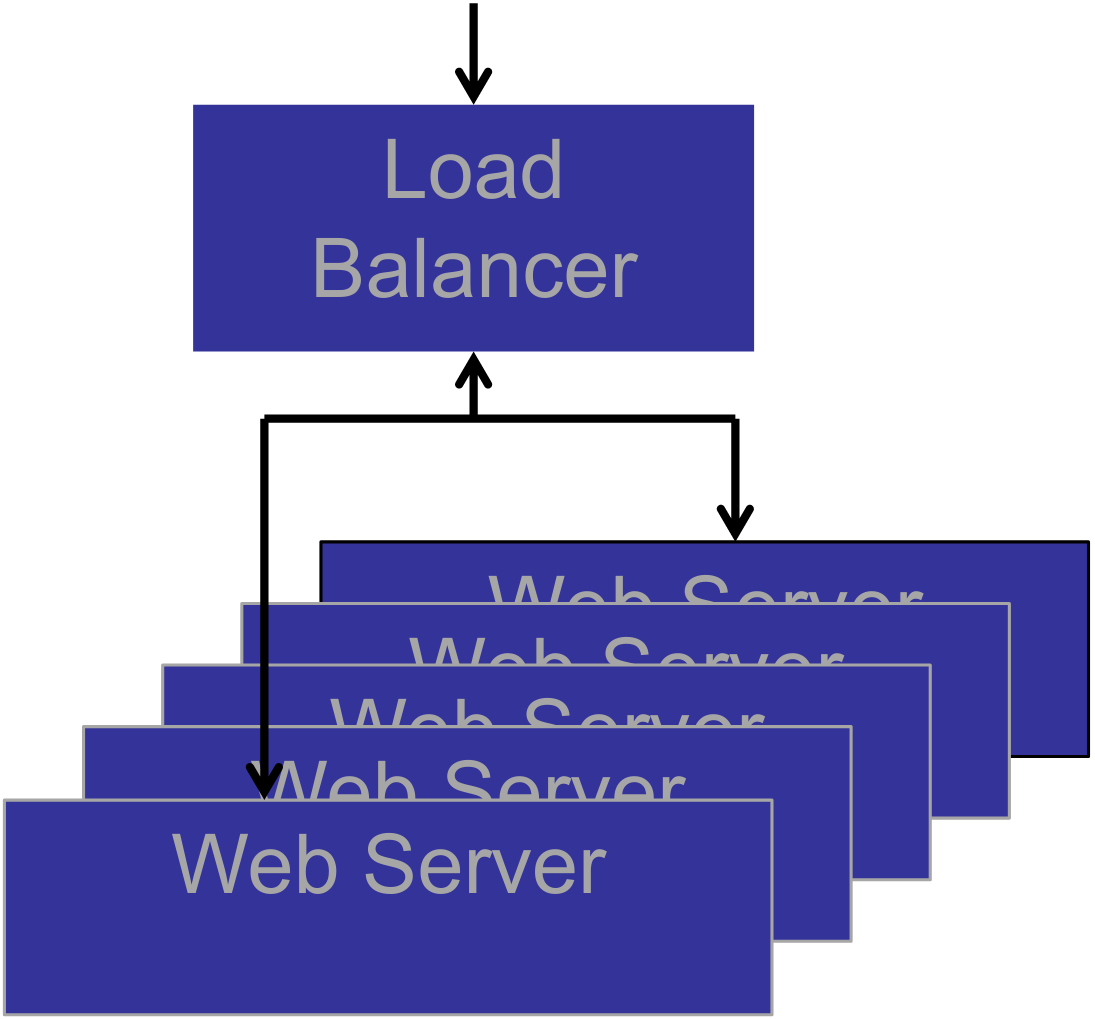
\includegraphics[height=150px]{ClusterMitLoadBalancer.png}

In dieser Architektur haben wir eine Vielzahl von gleichwertigen Servern, auf die Aufgaben verteilt werden können. Anfragen werden zunächst immer an einen Vermittler, den Load-Balancer, geschickt. Dieser entscheidet dann mittels eines simplen Verfahrens (z.B. Round-Robin), welcher Server des Clusters die Anfrage bearbeiten soll. Dadurch wird der Rechner, an den die Anfragen gesendet werden, entlastet. Dennoch werden alle Anfragen von nur einem Rechner bearbeitet, sodass dieser zum Bottleneck werden kann. Eine Möglichkeit das zu bewältigen sehen wir im Kapitel über \hyperref[client-based]{Client-Basierte Verfahren}. Außerdem ist das Gesamtsystem lahmgelegt, wenn bloß der Load Balancer ausfällt. Das kann einfach bewältigt werden, indem ein \hyperref[sec:fail-over-cluster]{Fail-Over-Cluster} für den Load-Balancer eingerichtet wird.\\
Ein weiteres Problem entsteht, wenn von den Clustern des Servers auch Daten geschrieben werden sollen. Dann müssten sofort die Daten auf den anderen Servern synchronisiert werden, um die Konsistenz beizubehalten.

\subsubsection{Server Cluster - n-Tier-Architektur}

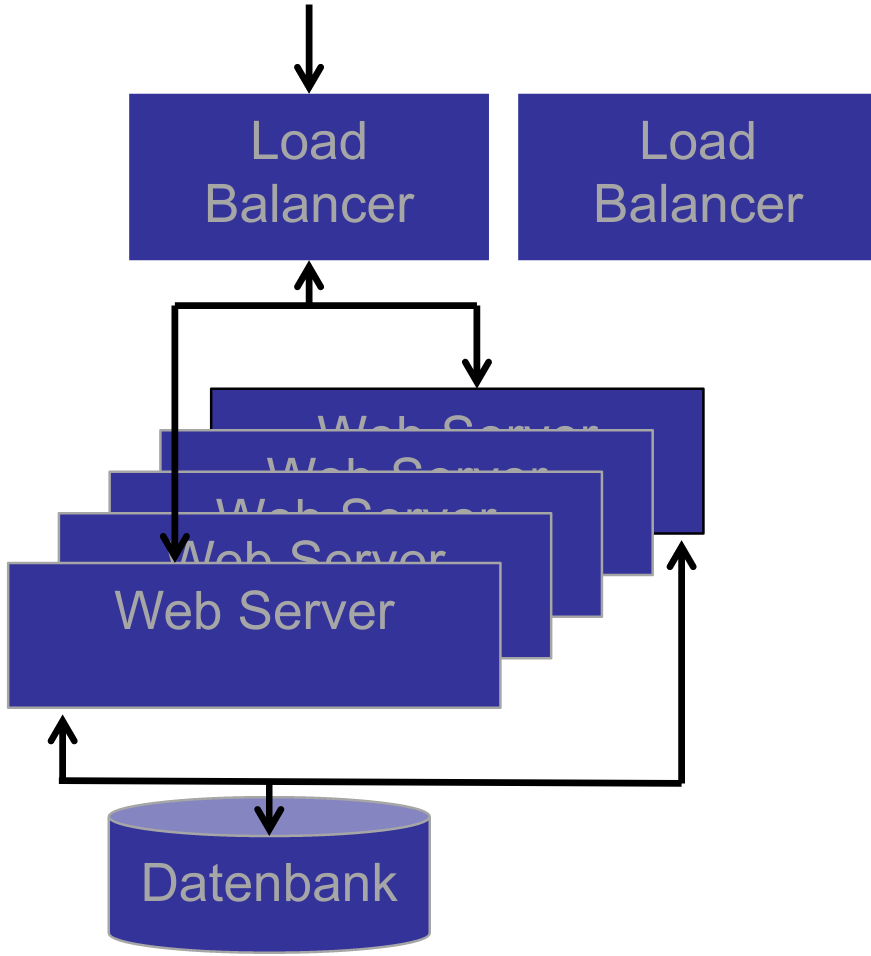
\includegraphics[height=150px]{n-tier-architektur.png}

Bei einer n-Tier-Architektur wir in der untersten Schicht mit einer gemeinsamen Datenquelle gearbeitet, um inkonsistenzen zu vermeiden. Somit sind, im Gegensatz zu einem \hyperref[sec:classic-server-cluster]{klassischen Server-Cluster}, auch Schreibzugriffe ohne inkonsistenzen möglich. Allerdings kann so die DB zum Bottleneck werden, weshalb viele DBMS schon von sich aus eine intelligentes Clustering implementieren.

\subsubsection{Server Cluster - Master-Slave}
\label{sec:master-slave}

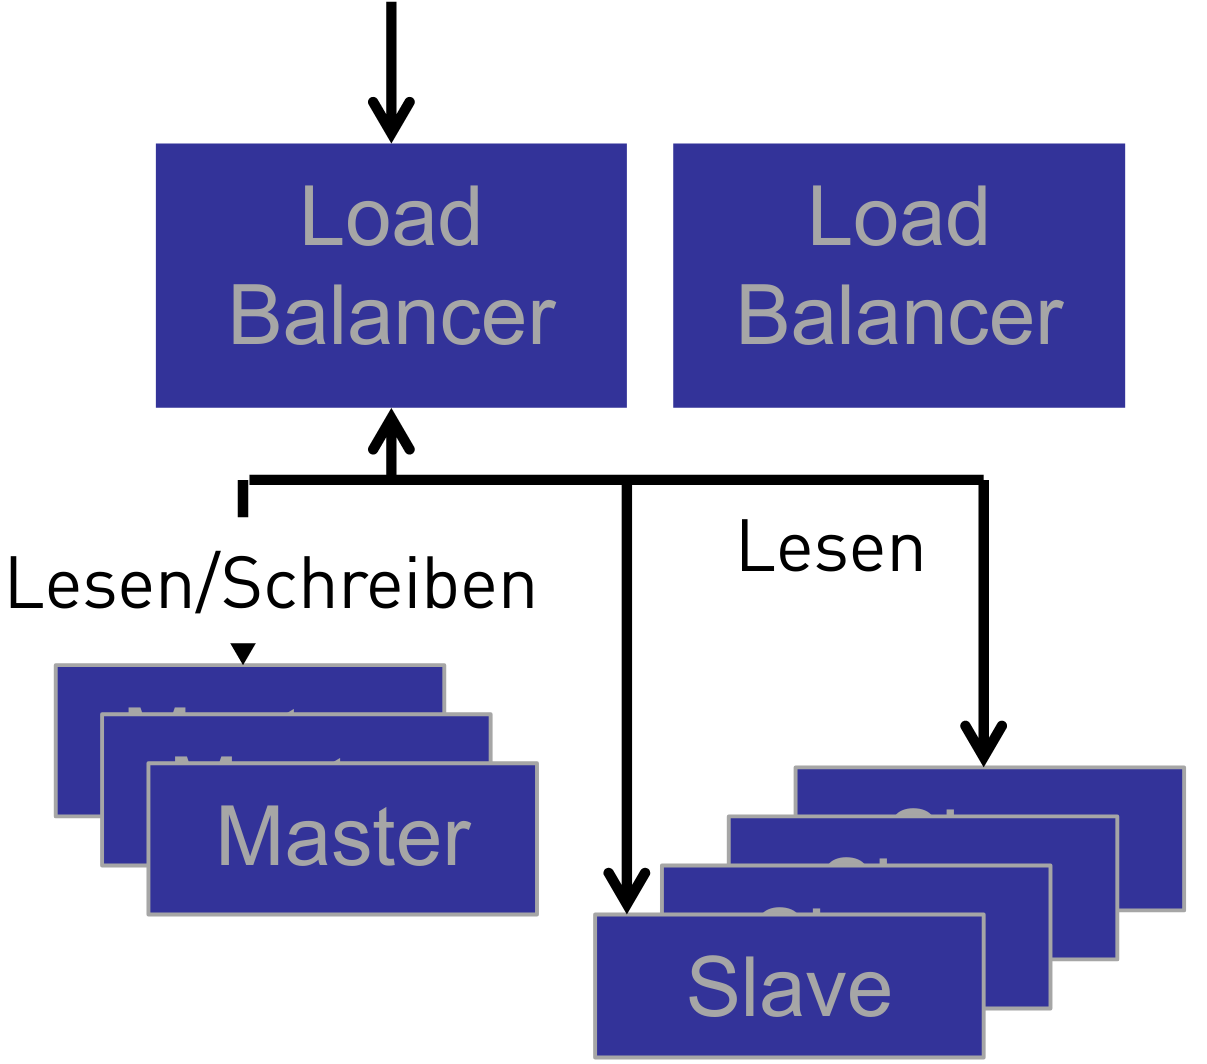
\includegraphics[height=150px]{MasterSlave.png}

In vielen Systemen sind Lesezugriffe deutlich häufiger als Schreibzugriffe. Dann bietet sich eine Master-Slave-Architektur an. Es gibt Master, die lesen und schreiben dürfen und Slaves, dei nur lesen dürfen. Wenn eine Master Daten verändert, dann sorgt er dafür, dass die Daten mit den Slaves synchronisiert werden. Auf diese Weise kann die Kommunikation zwischen den replizierten Servern verringert werden, da bekannt ist an welchen Knotenpunkten sich Daten ändern können.

\textbf{Verteilte Mater-Slaves:}\\
Eine andere Implementierungsvariante ist, dass jeder Server ein Master mit exklusivem Schreibzugriff für einen Bestimmten Teil der Daten ist. Auf diese Weise kann es zu keinen Schreib-anomalien mehr kommen, da in jedem Fall der eine schreibende Master der einzige ist, der diese Daten schreibt und damit die Daten auf diesem Master immer aktuell sind. Dennoch muss der Master nach einem Schreibzugriff die Daten auf die anderen Server verteilen, damit die Lesezugriffe von dort aus konsistent sind. Verteilte Mater-Slave Architekturen sind besonders skalierbar, da die Daten in beliebig viele Partitionen aufgeteilt werden können.

\textbf{Hashing:}
Die Load-Balancer müssen wissen auf welchen Server eine Anfrage umgeleitet werden soll. Das kann recht einfach mit Hash-Funktionen geschehen. Z.B. könnte man sich den Zugriff auf eine DB mit einem Primärschlüssel von integralem Typ vorstellen. Dann könnte eine Hashfunktion eine ID dieser DB mittels Modulo n auf n gleich große Gruppen aufteilen.



\subsubsection{Client-basierte Verfahren}
\label{client-based}

Wir können uns auch den Load-Balancer in einem \hyperref[sec:classic-server-cluster]{klassichen Server Cluster} sparen, indem wir die nötige Verteilungslogik in den Clients implementieren. Wenn z.B. jeder Client die Adresse aller Server, die einen Dienst anbieten, kennt, kann er einen zufälligen Server aussuchen, um so die Serverlast zu verteilen.\\
Eine mögliche Implementierung kann mithilfe von DNS SRVs (Service Records) erfolgen. In diesen Records können für einen Service die IP-Adressen aller Server eingetragen werden, die ihn anbieten. Dieses Verfahren wird z.B. beim SIP Protokoll für Voice-Over-IP verwendet.

\subsubsection{Map-Reduce-Verfahren}
\label{sec:map-reduce}

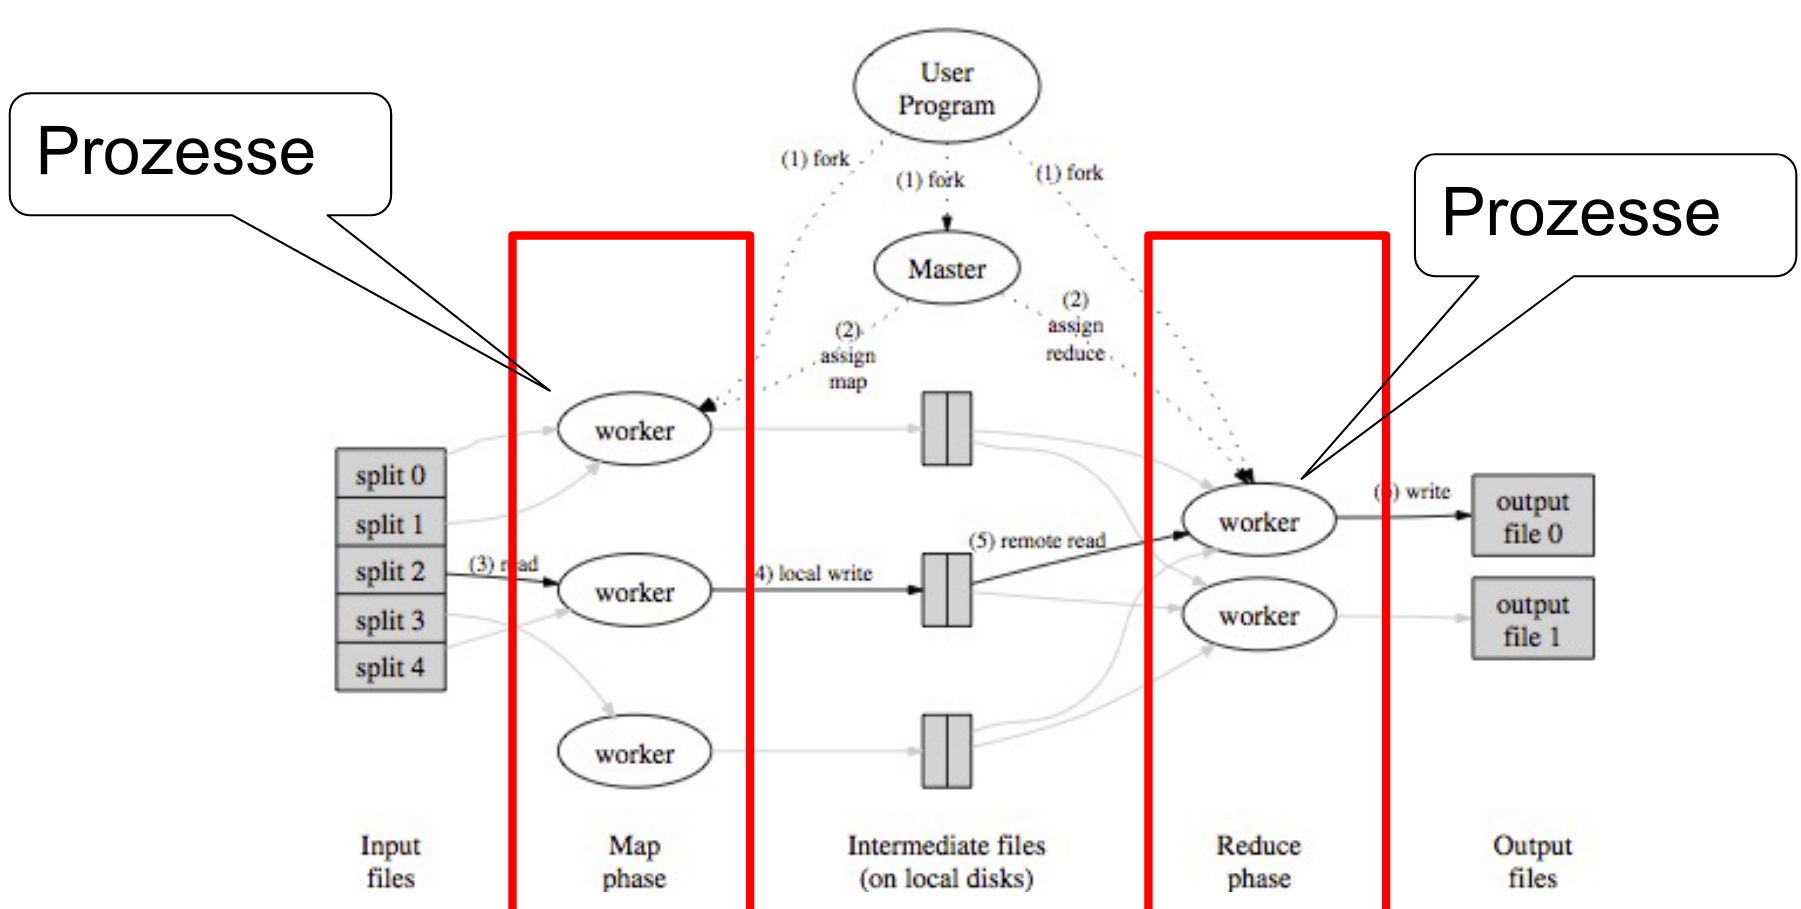
\includegraphics[height=200px]{map-reduce.png}

Map-Reduce ist ein von Google entwickeltes Verfahren zur Lastaufteilung bei CPU-intensiven Operationen. Das heißt hier geht es nicht darum möglichst viele Anfragen zu bewältigen, sonder eine Anfrage, die unglaublich viel Rechenpower benötigt, parallel auszuführen.\\
Bei diesem Verfahren werden die Eingangsdaten in gleichartige, ungefähr gleich aufwendige Pakete unterteilt. Jedes Paket wird an einen Worker verteilt. Die Worker machen den Job, der im Anwendungskontext, ausgeführt werden soll und verpacken das Ergebnis in key-value-Paare (map-phase). Dabei entstehen die sogenannten intermediate files, die dann in der reduce phase von separaten Prozessen zu einem Gesamtergebnis akkumuliert werden sollen.\\
Dieses Verfahren ist sehr einfach und unbegrenzt skalierbar. Allerdings ist es auch nur für eine bestimmt Gruppe von Problemen anwendbar. Nämlich für solche, bei denen ein Problem in unabhängige Teilprobleme, also solche bei denen keine Kommunikation zwischen den Workern notwendig ist, unterteilt werden kann. Zusätzlich muss es möglich sein, die Teilergebnisse als Key-Value Paare darzustellen und diese dann zu akkumulieren. Die Logik in der Map- und Reduce-Phase muss also gut durchdacht sein. Ein Anwendungsbeispiel ist etwa bei Suchmaschinen das durchsuchen vieler Millionen Texte nach einem Schlüsselwort. Jeder Worker übernimmt dann eine bestimmte Anzahl von Texten. Das Ergebnis der Map-Phase sind einzelne key-value-Paare, die z.B. aus der URL zum durchsuchten Text und der Häufigkeit des gesuchten Wortes bestehen. In der Reduce-Phase wäre in diesem Fall nicht mehr zu tun als die Ergebnisse der Map-Phase gesammelt zurückzugeben.\\

Dienste, die Map-Reduce anbieten, sind z.B.:
\begin{itemize}
    \item Amazon Elastic Map Reduce
    \item Google App Engine
    \item Bibliothek: Apache Hadoop
\end{itemize}

\textbf{Variante: Apache Spark}\\
Apache Spark ist eine Open-Source-Lib, die darauf ausgelegt ist, mehrere iterationen von Map-Reduce hintereinander durchzuführen. Dabei können die Ergebnisse der einzelnen Iterationen im HS zwischengespeichert werden und von den nächsten Iterationen abgerufen werden. Verglichen mit klassischem Map-Reduce (z.B. Hadoop) ist Spark je nach Anwendungsfall möglicherweise deutlich schneller. Allerding können in Hadoop deutlich größere Datenmengen verarbeitet werden, da die Daten über das Dateisystem geladen werden.


\subsection{Pipelining \& Interner Serveraufbau}

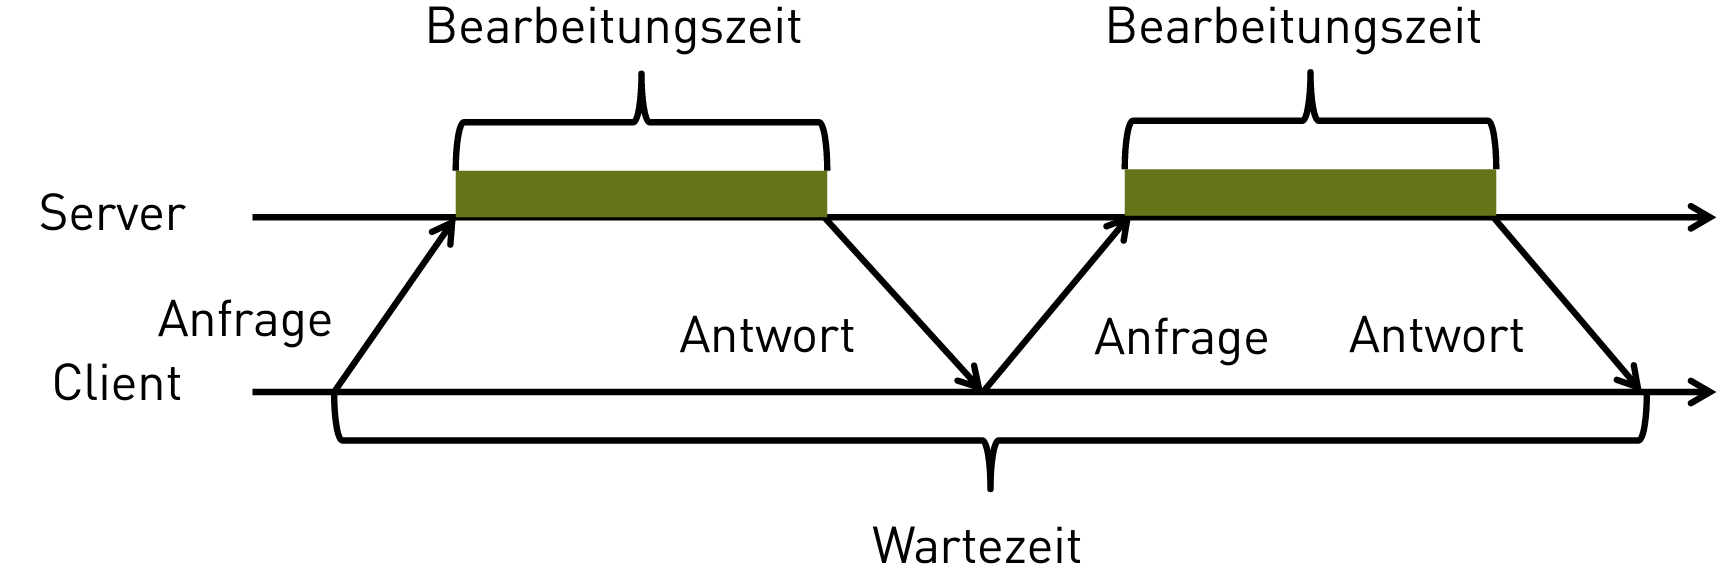
\includegraphics[width=300px]{pipelining1.png}

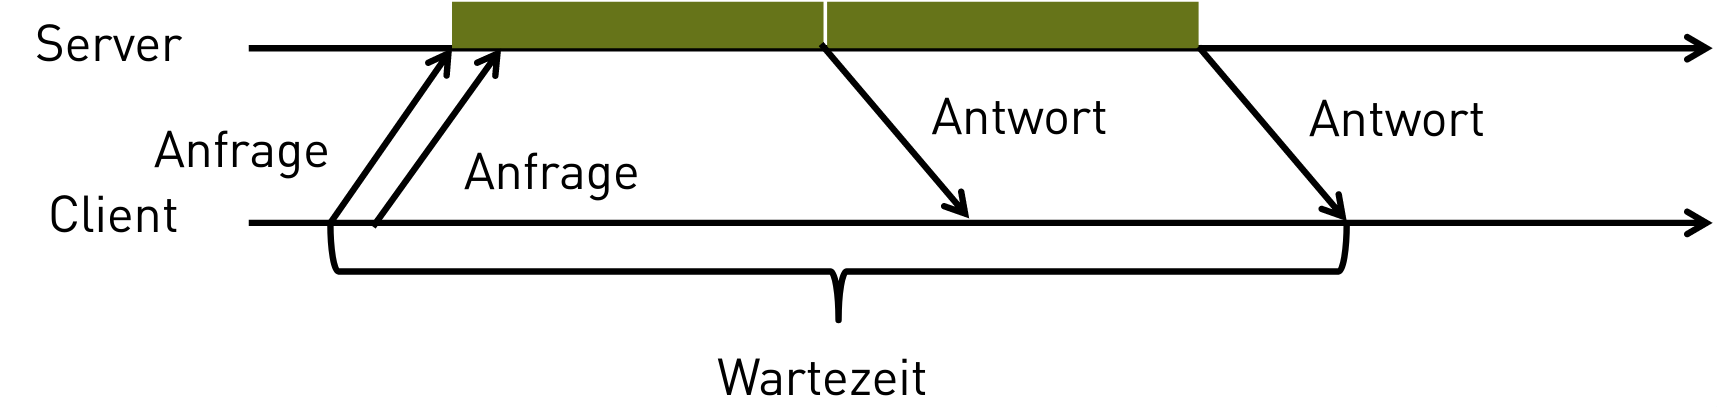
\includegraphics[width=300px]{pipelining2.png}

Im oberen Bild können wir sehen, dass der Client nach dem Senden einer Nachricht auf die Antwort wartet und dann erst die zweite Anfrage sendet. Manche Protokolle (z.B. Http 1.1) unterstützen aber auch die Möglichkeit mehrere Anfragen zu schicken ohne auf die Antwort der vorherigen Anfrage zu warten. Auf diese Weise hat der Server weniger Leerlauf und die Antworten treffen mit weniger Wartezeit beim Client ein.\\

Intern arbeiten die Server allerdings auch oft mit mehreren Threads. Ist das der Fall, so muss Pipelining nicht mehr beachtet werden, da jede Anfrage ohnehin von einem anderen Thread behandelt wird.